\section{Experiments}
\begin{frame}
\frametitle{Experiments---Progressive Modeling Scaling}
\begin{figure}[h]
    \centering
    \begin{minipage}{0.49\linewidth}
        \centering
        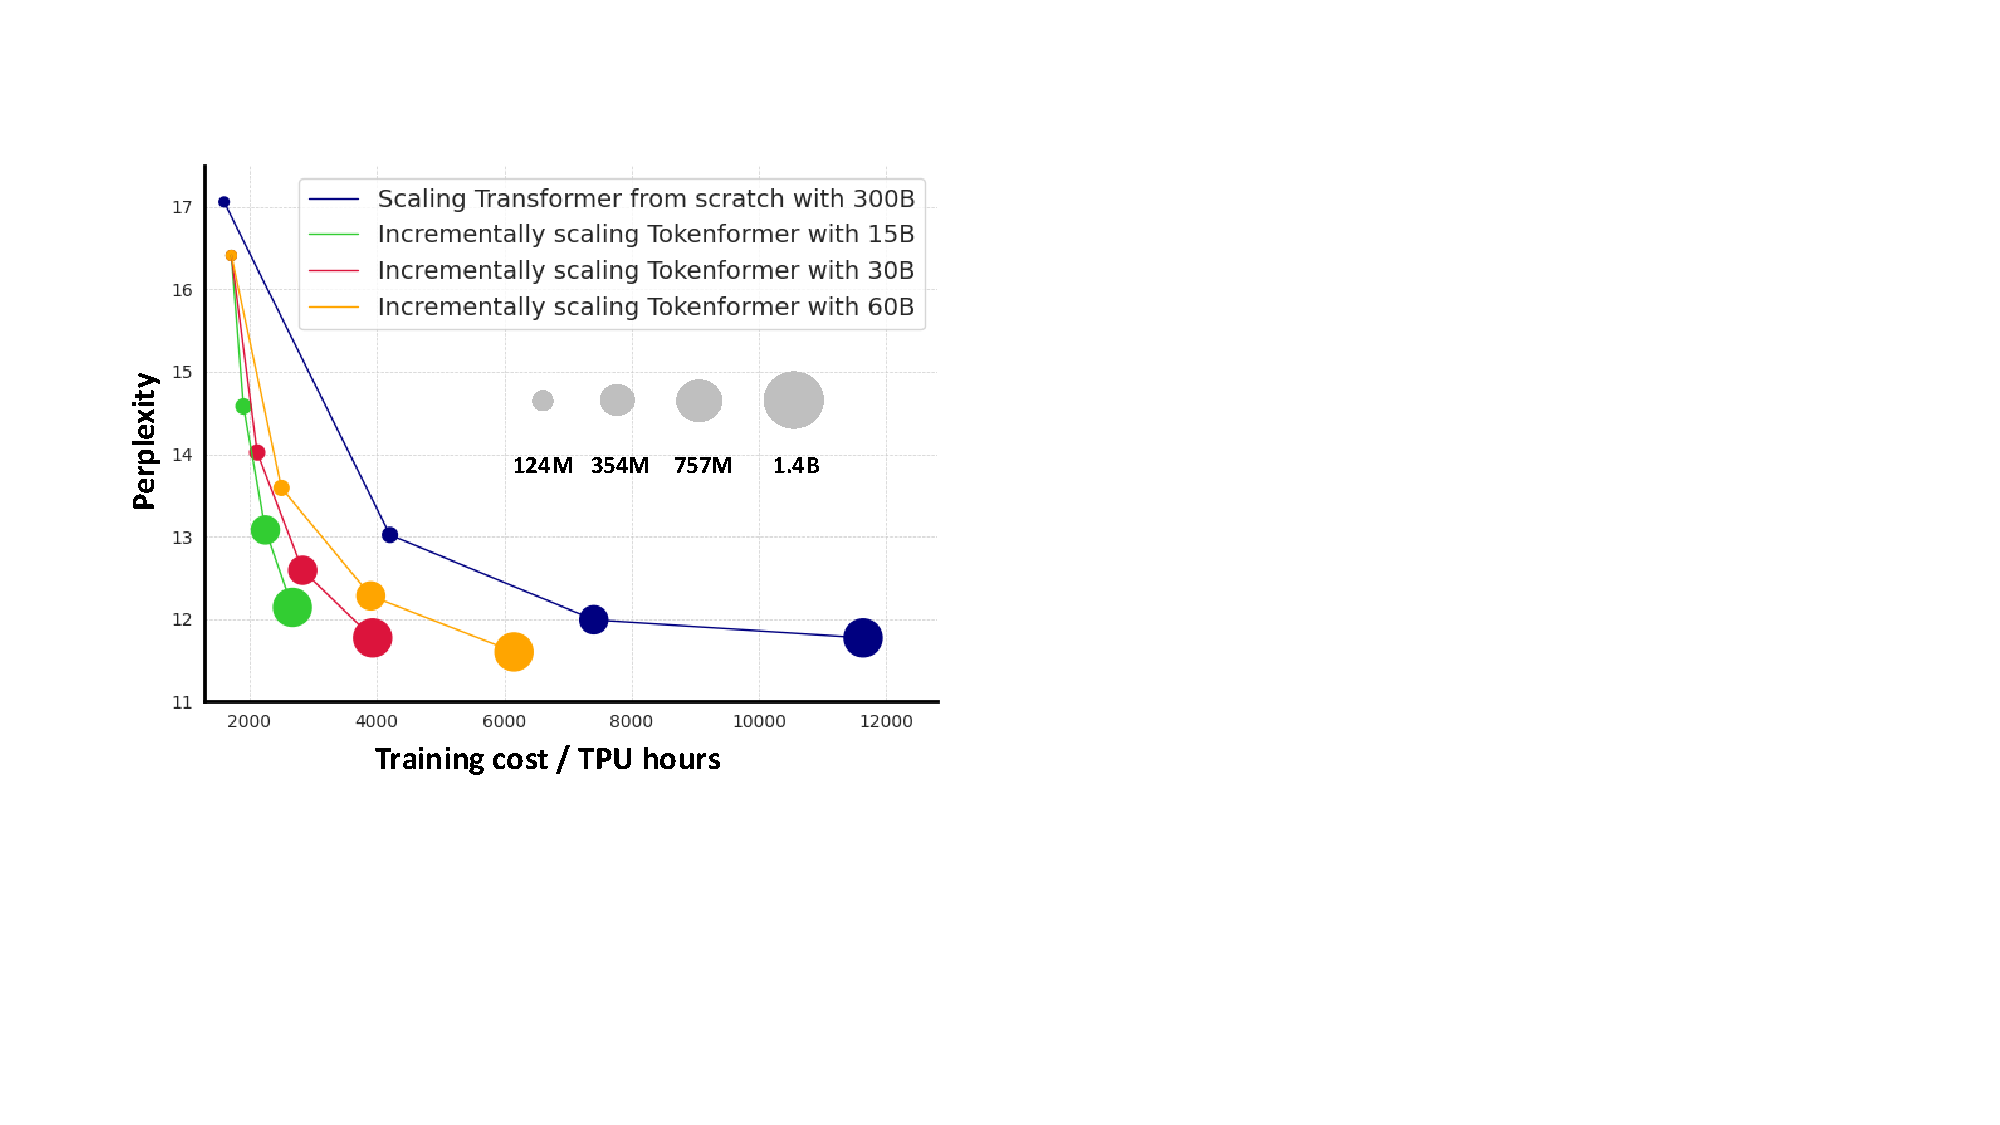
\includegraphics[width=1.0\linewidth]{./transformer-paper/main_results_v2_left.pdf}
        %\vspace{-16pt}
        %\caption{Evaluating model scaling costs through cumulative computational budgets. The Transformer baseline incurs expenses for each individual scaling step performed independently from scratch, whereas \ourmethod aggregates costs across all scaling stages, including training a 124M model initially, progressively scaling to 354M, 757M, and 1.4B parameters.}
        \label{fig:scaling_accum}
    \end{minipage}
    \hfill
    \begin{minipage}{0.49\linewidth}
        \centering
        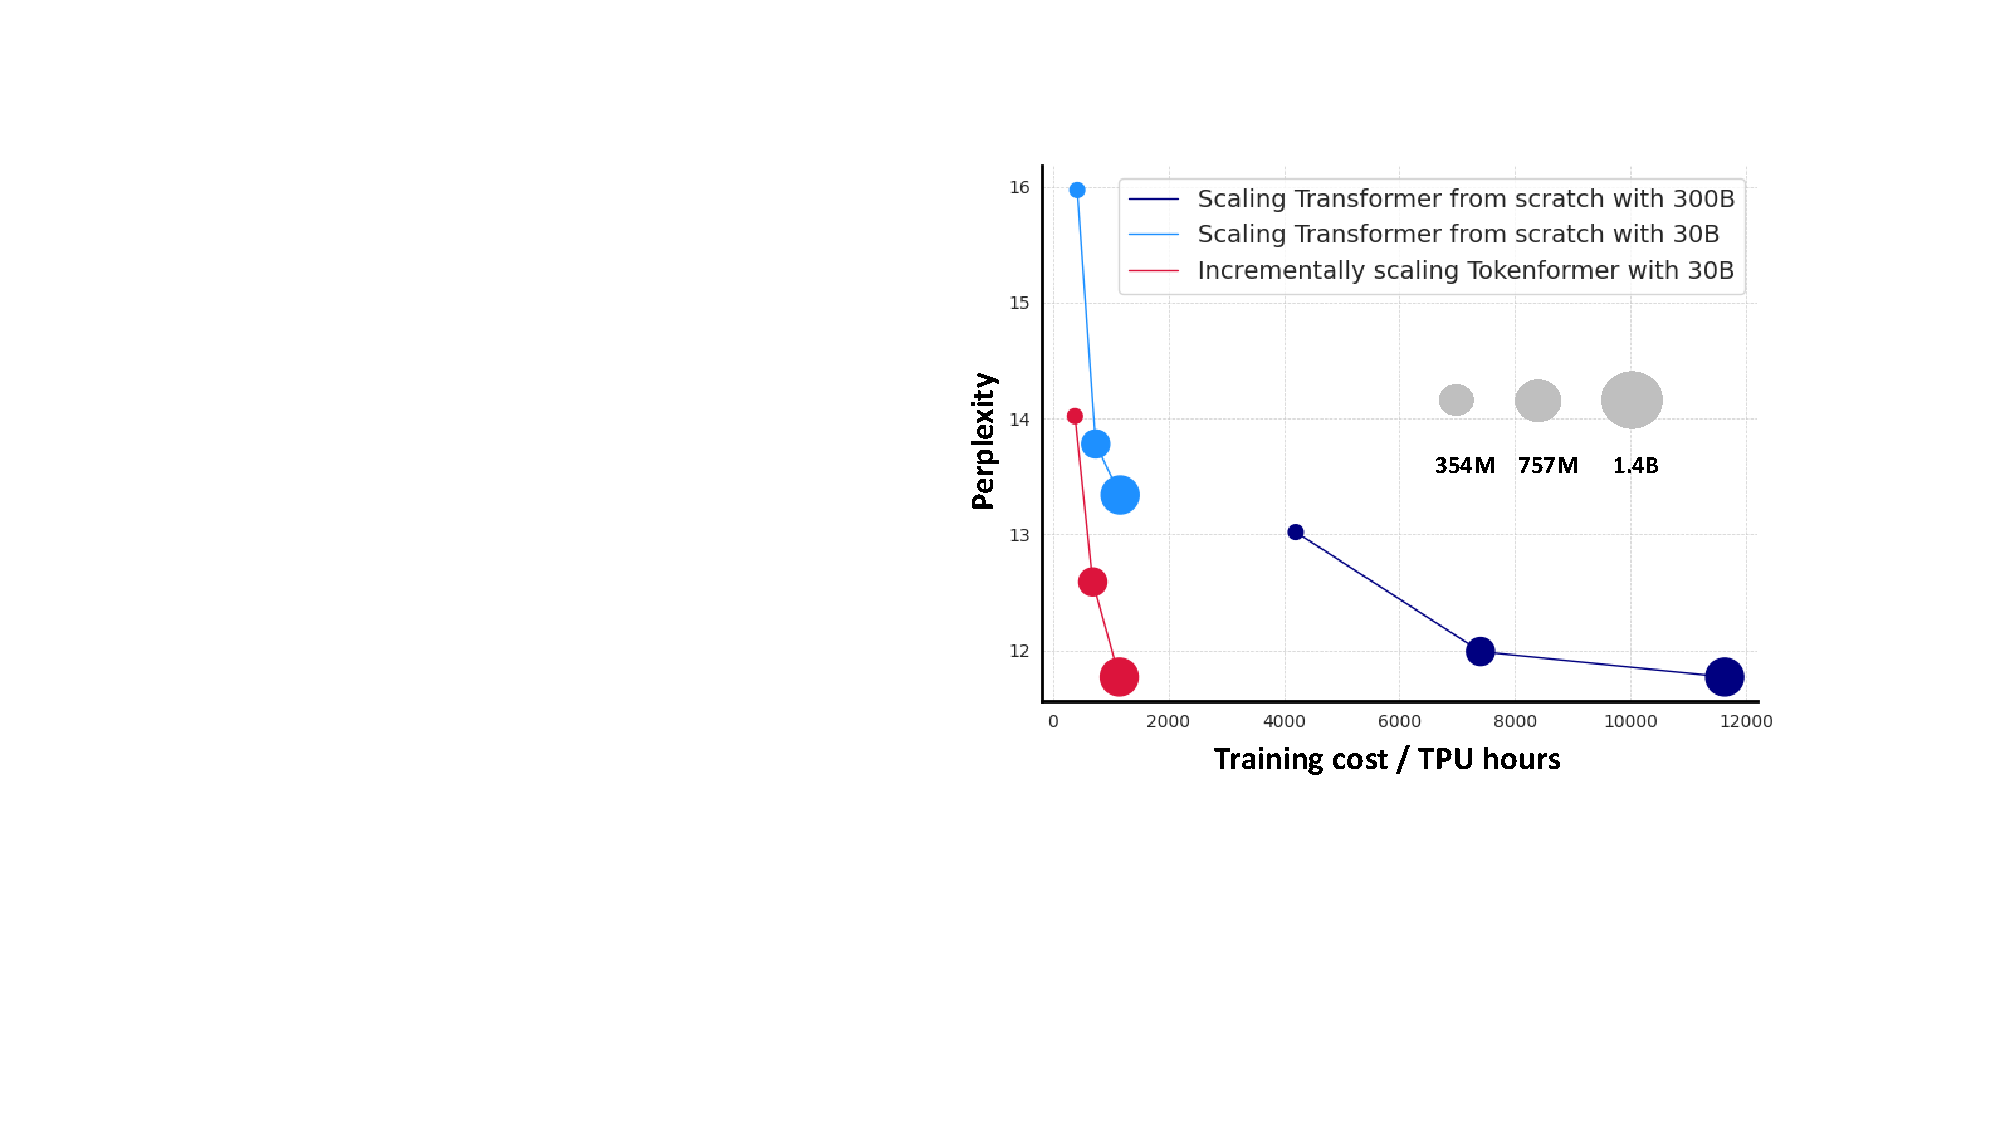
\includegraphics[width=1.0\linewidth]{./transformer-paper/main_results_v2_right.pdf}
        %\vspace{-16pt}
        %\caption{Evaluating model scaling costs by measuring the budget required at each scaling stage. The Transformer baselines used are consistent with those depicted in Figure~\ref{fig:scaling_accum}, trained with 30B and 300B tokens. Similarly, for \ourmethod, the cost is the budget required for each incremental scaling step from a smaller one. All the experiments were conducted on TPU v4 hardware.}
        \label{fig:scaling_individual}
    \end{minipage}
\end{figure}
\end{frame}

\begin{frame}
\frametitle{Experiments---Benchmarking}
\begin{table}[t]
    \centering
    \resizebox{\textwidth}{!}{
    \begin{tabular}{cccccccccc|c}
      \toprule
      & & Pile & LAMBADA & LAMBADA & HellaSwag & PIQA & Arc-E & Arc-C & WinoGrande & Average \\
      \multirow{-2}{*}{Model}     & \multirow{-2}{*}{\#Param}    & ppl $\downarrow$ & ppl $\downarrow$ & acc $\uparrow$ & acc $\uparrow$ & acc $\uparrow$ & acc $\uparrow$ & acc $\uparrow$  & acc $\uparrow$ & acc $\uparrow$\\
      \midrule
      Pythia-160M 			& 160M	   & 29.64 & 37.25 & 35.4 & 30.3 & 62.3 & 43.6 & 23.6 & \textbf{51.3} & 40.1\\
      \textbf{Ours (TokenFormer-150M)} & 150M & \textbf{10.45} & \textbf{16.38} & \textbf{45.0} & \textbf{35.5} & \textbf{64.9} & \textbf{47.3} & \textbf{24.9} & 50.4 & \textbf{44.7}\\
      \midrule
      Pythia-410M 			& 410M	   & 9.95 & 10.84 & 51.4 & 40.6 & 66.9 & 52.1 & 24.6 & 53.8 & 48.2\\
      \textbf{Ours (TokenFormer-450M)}			    & 450M	   & \textbf{8.28} & \textbf{7.69} & \textbf{57.3} & \textbf{47.5} & \textbf{69.5} & \textbf{56.2} & \textbf{26.7} & \textbf{54.6} & \textbf{52.0}\\
      \midrule
      Pythia-1B 			& 1B	   & 7.82 & 7.92 & 56.1 & 47.2 & 70.7 & 57.0 &  27.1 &  53.5 & 51.9\\
      \textbf{Ours (TokenFormer-900M)}			    & 900M	   & \textbf{7.38} & \textbf{5.46} & \textbf{64.0} & \textbf{55.3} & \textbf{72.4} & \textbf{59.9} &  \textbf{30.6} &  \textbf{56.4} & \textbf{56.4} \\
      \midrule
      GPT-Neo 1.3B           & 1.3B     &  -   &7.50 & 57.2 & 48.9 & 71.1 & 56.2 & 25.9 & 54.9 & 52.4 \\
      OPT-1.3B            & 1.3B     &  -   &6.64 & 58.0 & 53.7 & 72.4 & 56.7 & 29.6 & 59.5 & 55.0 \\
      Pythia-1.3B			& 1.3B	   & 7.51 &6.08 & 61.7 & 52.1 & 71.0 & 60.5 &  28.5 &  57.2 & 55.2\\
      GPT-Neo 2.7B            & 2.7B     &  -   &5.63 & 62.2 & 55.8 & 71.1 & 61.1 & 30.2  & 57.6 & 56.5\\
      OPT-2.7B            & 2.7B     &  -   &5.12 & 63.6 & \textbf{60.6} & 74.8 & 60.8 & 31.3 & \textbf{61.0} & 58.7\\
      Pythia-2.8B			& 2.8B	   & - &\textbf{5.04} & 64.7 & 59.3 & 74.0 & 64.1 &  \textbf{32.9} &  59.7 & 59.1\\
      \hline
      \textbf{Ours (TokenFormer-1.5B)}			& 1.5B	   & \textbf{6.91} & 5.24 & \textbf{64.7} & 60.0 & \textbf{74.8} & \textbf{64.8} &  32.0 & 59.7 & \textbf{59.3} \\
      \bottomrule
    \end{tabular}
    } 
    %\vspace{-8pt}
      \caption{\textbf{Zero-shot Evaluations.}}
      % The best performance for each model size is highlighted in bold. Our comparisons are made with publicly available transformer-based LMs with various tokenizers. Following Pythia~\citep{biderman2023pythia}, our model is trained for up to 300B tokens on pile dataset. }
      \label{tab:llm_benchmark}
  \end{table}
\end{frame}

\begin{frame}
\frametitle{Experiments---Benchmarking}
\begin{table}[t]
    \vspace{-2pt}
    \centering
    \resizebox{0.6\textwidth}{!}{
    \begin{tabular}{cccccccccc}
      \toprule
     Method & Image Size &  \#Param&Top-1 acc \\
      \midrule
      ViT-B/16 			& 384$^2$ & 86M  & 77.9\\
      DeiT-B/16			& 224$^2$ & 86M  & 81.8\\
      ViT-B/16~(MAE) 			& 224$^2$ & 86M  & 82.3\\
      Ours (TokenFormer-B/16$^{\dag}$ )			& 224$^2$ & 86M  & 82.1\\
      \textbf{Ours (TokenFormer-B/16)}			& 224$^2$ & 109M & \textbf{82.5}\\
      \midrule
      ViT-L/16 			& 384$^2$ & 307M & 76.5\\
      ViT-L/16~(MAE)			& 224$^2$ & 307M & 82.6\\
      Ours (TokenFormer-L/16$^{\dag}$)			& 224$^2$ & 307M & 83.0 \\
      \textbf{Ours (TokenFormer-L/16)}			& 224$^2$ & 407M & \textbf{83.1} \\
      \bottomrule
    \end{tabular}
    }
  \caption{\textbf{Image Classification.}} 
  %Comparison of standard vision transformer on ImageNet-1K. The training hyperparameters are completely consistent~(batch size, learning rate, etc.) with \citet{he2022masked}. $\dag$ denotes models where the parameter size has been matched to that of the standard ViT.}
  \label{tab:visual_benchmark}
  %\vspace{-8pt}
\end{table}
\end{frame}

\begin{frame}
\frametitle{Experiments---Comparison with Transformer}
\begin{table}[h]
  \centering
  \resizebox{\textwidth}{!}{
  \begin{tabular}{lcc|cc}
    \toprule
    & \multicolumn{2}{c}{Parameter~~~~~~~~~~~~~~~} & \multicolumn{2}{c}{Training FLOPs}\\
    \multirow{-2}{*}{Operation} & Transformer & Ours & Transformer & Ours \\
    \midrule
    Embed  		& $n_{\text{vocab}}d_{\text{model}}$  & $n_{\text{vocab}}d_{\text{model}}$ & - & -\\
    Attention: QKV Project  		& $3n_{\text{layer}}d_{\text{model}}^2$  & $n_{\text{layer}}d_{\text{token}}(n_{\text{q}}+ n_{\text{k}} + n_{\text{v}}$)& $6n_{\text{layer}}d_{\text{model}}^2T$& $2n_{\text{layer}}d_{\text{token}}(n_{\text{q}}+ n_{\text{k}} + n_{\text{v}})T$\\
    Attention: Token-Token 		& - & - & $4n_{\text{layer}}d_{\text{model}}T^2$ & $4n_{\text{layer}}d_{\text{token}}T^2$ \\
    Attention: Output Project      & $n_{\text{layer}}d_{\text{model}}^2$ & $n_{\text{layer}}d_{\text{token}}n_{\text{o}}$ & $2n_{\text{layer}}d_{\text{model}}^2T$ & $2n_{\text{layer}}d_{\text{token}}n_{\text{o}}T$\\
    Feedforward          & $8n_{\text{layer}}d_{\text{model}}^2$   & $2n_{\text{layer}}d_{\text{token}}n_{\text{ff}}$ & $16n_{\text{layer}}d_{\text{model}}^2T$ & $4n_{\text{layer}}d_{\text{token}}n_{\text{ff}}T$\\
    De-embed  		& - & - & 2$n_{\text{vocab}}d_{\text{model}}$ & 2$n_{\text{vocab}}d_{\text{model}}$\\
    \midrule
    Total~(Non-Embedding)           & $N=12n_{\text{layer}}d_{\text{model}}^2$    & $N=n_{\text{layer}}d_{\text{token}}(n_{\text{q}}+n_{\text{k}}+n_{\text{v}}+n_{\text{o}}+2n_{\text{ff}})$ & $2NT + 4n_{\text{layer}}d_{\text{model}}T^2$ & $2NT + 4n_{\text{layer}}d_{\text{token}}T^2$ \\
    \bottomrule
  \end{tabular}
  }
    \caption{Parameter counts and training compute estimates for Transformer and Tokenformer.}
    \label{tab:flops_and_param}
\end{table}
\end{frame}

\begin{frame}
\frametitle{Experiments---Comparison with Transformer}
\begin{figure}[h]
  \centering
  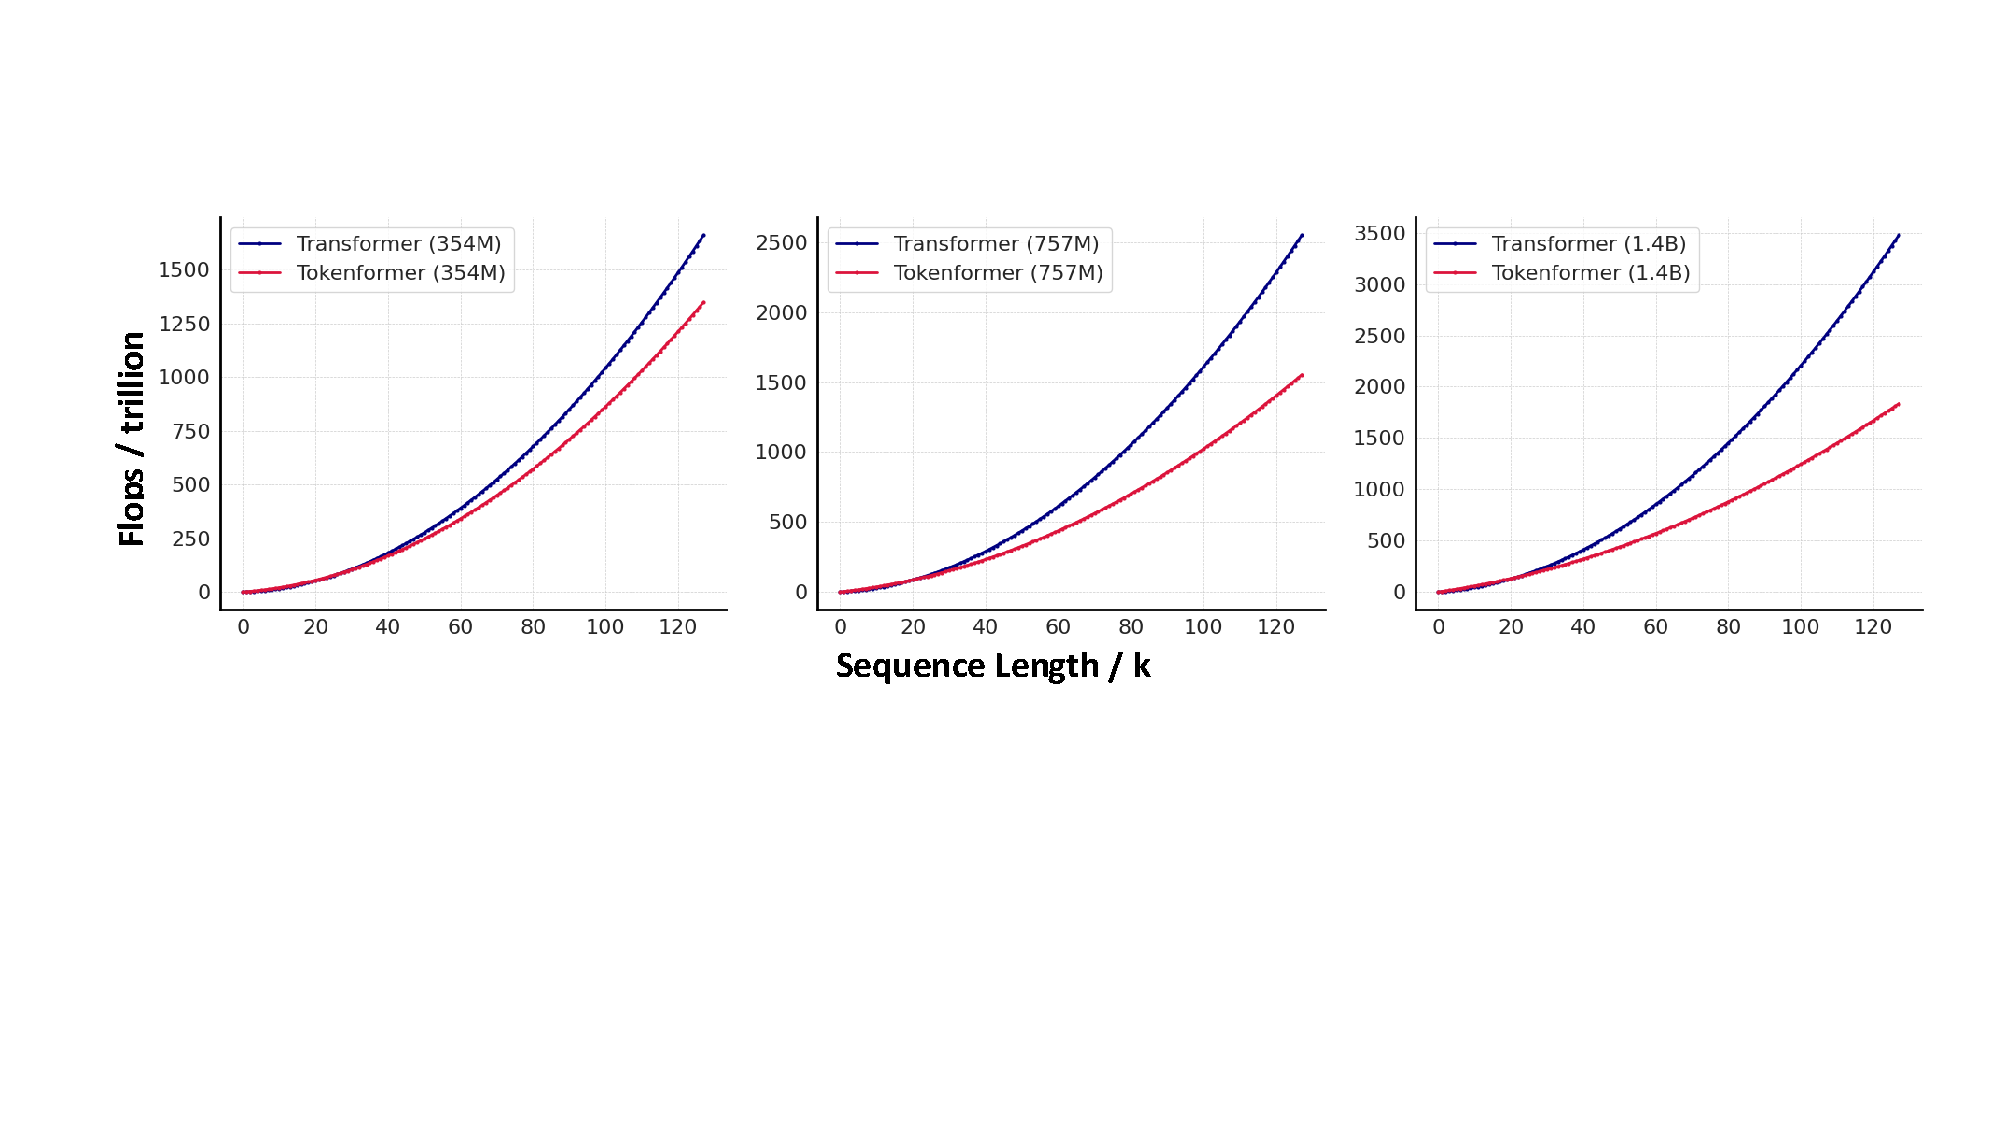
\includegraphics[width=\linewidth]{./transformer-paper/flops_figure.pdf}
  \caption{The relationship between FLOPs and text length for both Transformer and Tokenformer.}
    \label{fig:flops_figure}
\end{figure}
\end{frame}

\begin{frame}
\frametitle{Experiments---Comparison with Transformer}
\begin{figure}[t]
  \centering
  \begin{minipage}{0.49\textwidth}
      \centering
      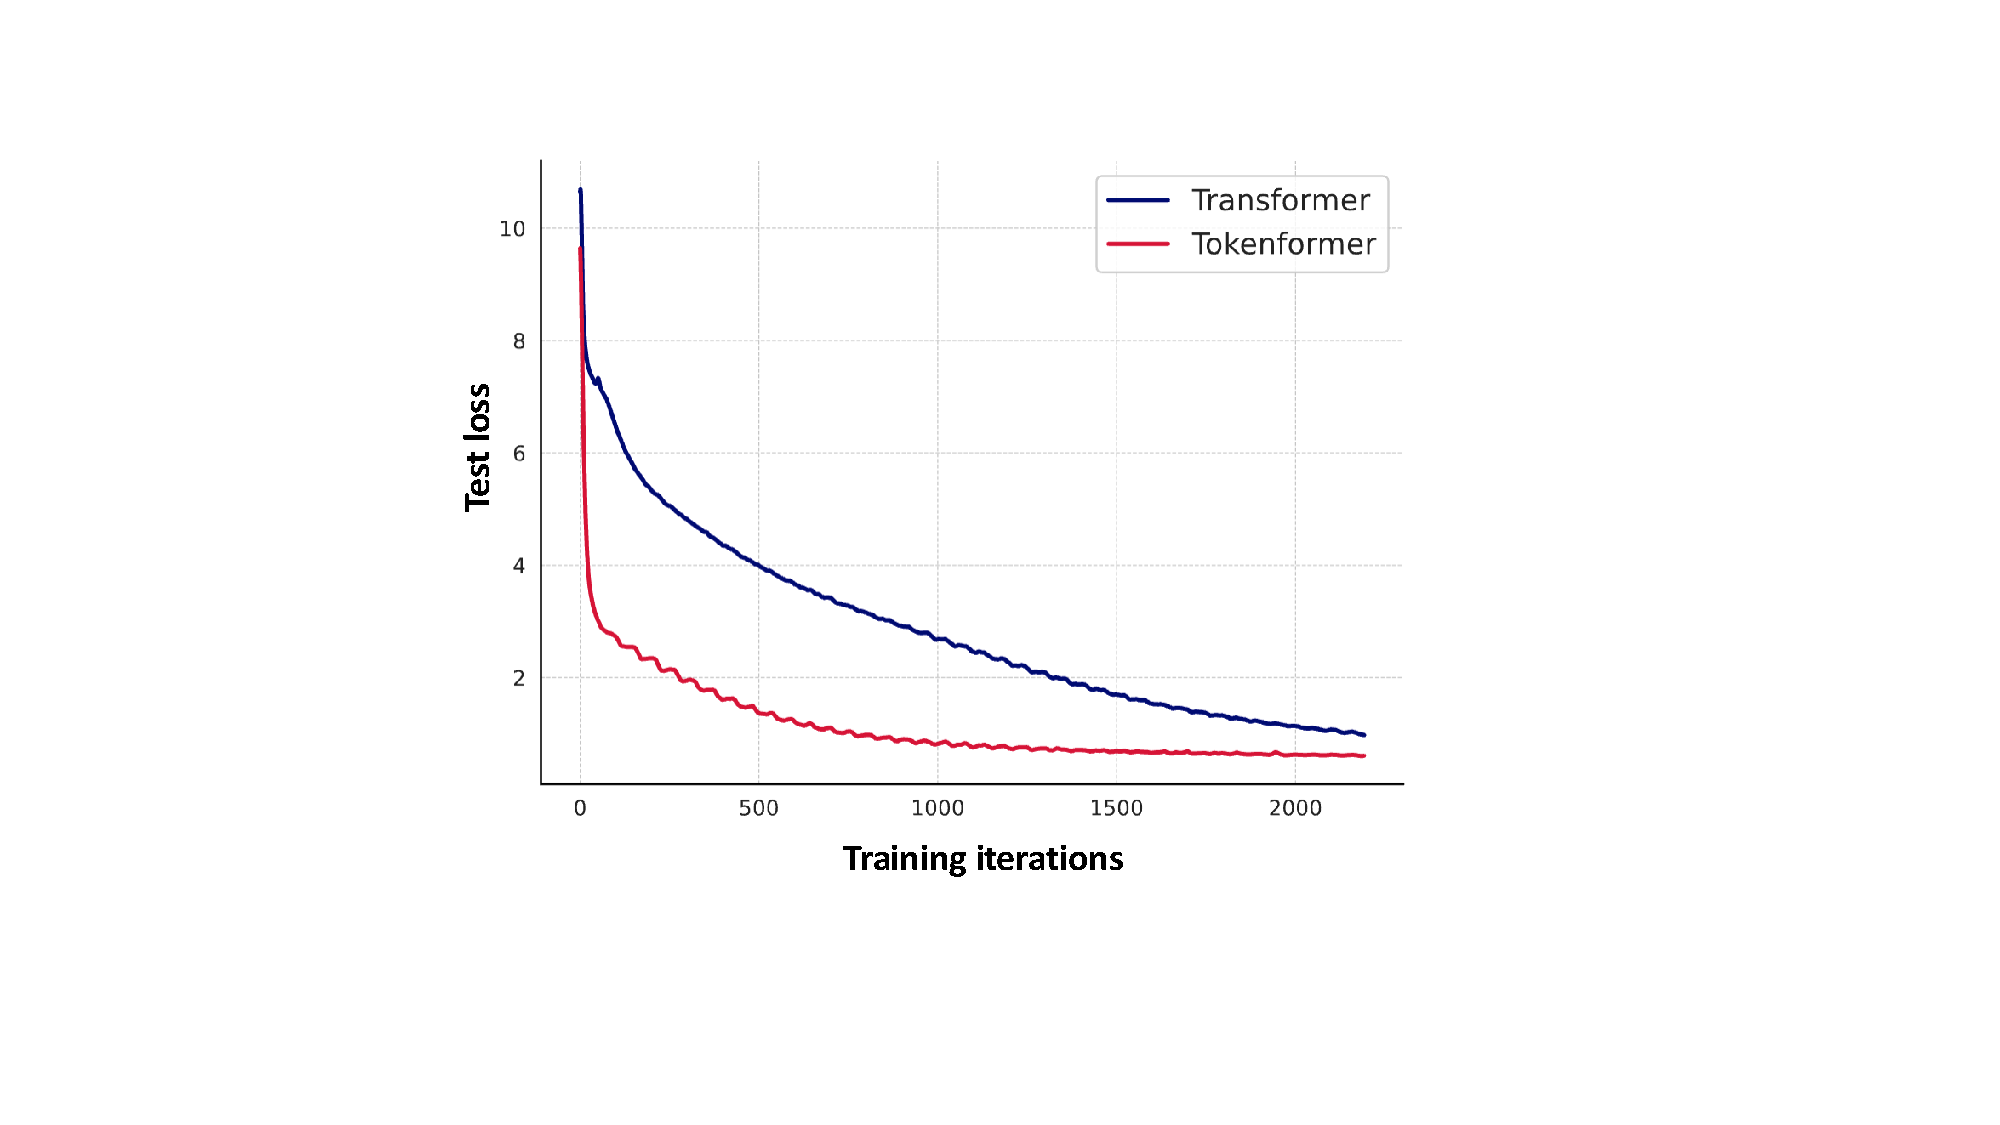
\includegraphics[width=\linewidth]{./transformer-paper/zero_init_v2.pdf}
      \caption{Loss curves comparing pre-trained Transformer and Tokenformer as their parameters are scaled during continued training on enwik8.}
      \label{fig:zero_init}
  \end{minipage}%
  \hfill
  \begin{minipage}{0.49\textwidth}
      \centering
      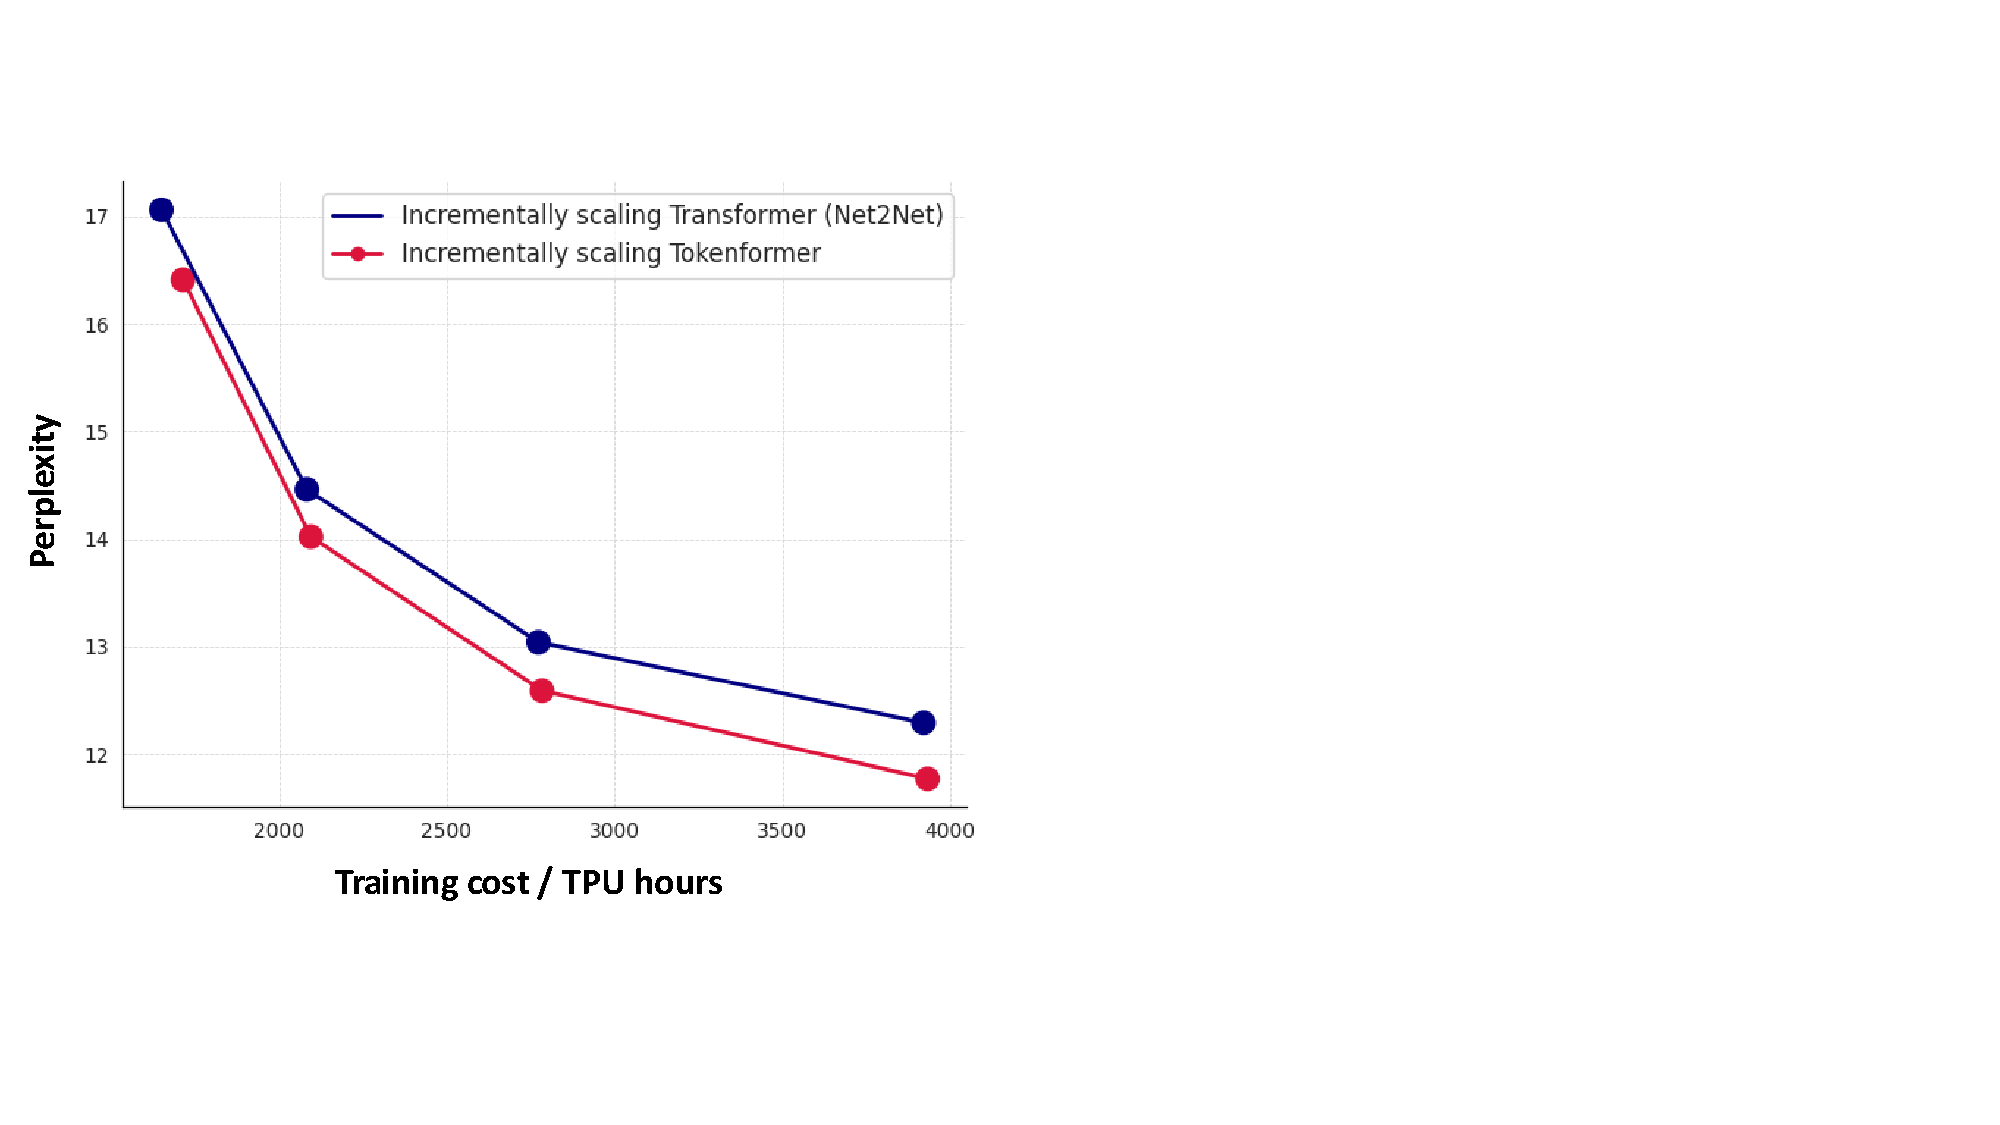
\includegraphics[width=\linewidth]{./transformer-paper/trans_vs_token.pdf}
      \caption{Performance benchmarking on incremental model scaling between Transformer with Net2Net scheme and Tokenformer.}
      \label{fig:comparision_tf_to}
  \end{minipage}
\end{figure}
\end{frame}

